\chapter{The Foundation of Mathematics: Addition and Subtraction}

\section{Introduction: The Power of Basic Operations}
Addition and subtraction form the cornerstone of mathematics. They are the fundamental operations that unlock the door to more complex mathematical concepts. In this chapter, we'll explore these operations in depth, understanding not just how to perform them, but why they work and how they apply to real-world situations.

\section{Understanding Addition}
\subsection{Definition and Concept}
Addition is the process of combining two or more quantities to form a new total. It's represented by the symbol '+'.

\begin{example}
If you have 3 apples and someone gives you 2 more apples, you now have 5 apples in total.
Mathematically: $3 + 2 = 5$
\end{example}

\subsection{Properties of Addition}
\begin{itemize}
    \item \textbf{Commutative Property:} The order of addends doesn't affect the sum.
    \[ a + b = b + a \]
    \item \textbf{Associative Property:} The grouping of addends doesn't affect the sum.
    \[ (a + b) + c = a + (b + c) \]
    \item \textbf{Identity Property:} Adding zero to any number doesn't change the number.
    \[ a + 0 = a \]
\end{itemize}

\subsection{Visualizing Addition}
A number line is an excellent tool for visualizing addition. To add, move right on the number line.

\begin{center}
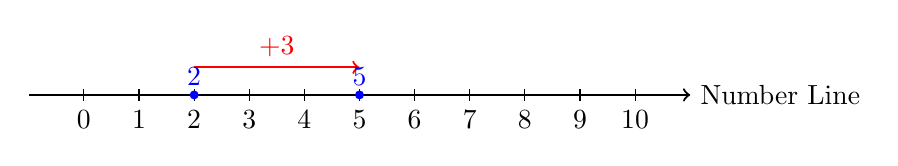
\begin{tikzpicture}[scale=0.7]
    \draw[thick,->] (-1,0) -- (11,0) node[right] {Number Line};
    \foreach \x in {0,1,...,10}
        \draw (\x,3pt) -- (\x,-3pt) node[below] {\x};
    \draw[red,thick,->] (2,0.5) -- (5,0.5) node[midway,above] {+3};
    \filldraw[blue] (2,0) circle (2pt) node[above] {2};
    \filldraw[blue] (5,0) circle (2pt) node[above] {5};
\end{tikzpicture}
\end{center}

\section{Mastering Subtraction}
\subsection{Definition and Concept}
Subtraction is the process of removing one quantity from another. It's represented by the symbol '-'.

\begin{example}
If you have 7 cookies and eat 3, you're left with 4 cookies.
Mathematically: $7 - 3 = 4$
\end{example}

\subsection{Properties of Subtraction}
\begin{itemize}
    \item \textbf{Non-Commutative:} The order matters in subtraction.
    \[ a - b \neq b - a \text{ (generally)} \]
    \item \textbf{Relationship to Addition:} Subtraction is the inverse of addition.
    \[ \text{If } a + b = c, \text{ then } c - b = a \]
\end{itemize}

\subsection{Visualizing Subtraction}
On a number line, subtraction is represented by moving left.

\begin{center}
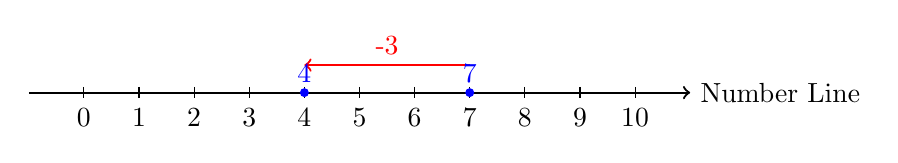
\begin{tikzpicture}[scale=0.7]
    \draw[thick,->] (-1,0) -- (11,0) node[right] {Number Line};
    \foreach \x in {0,1,...,10}
        \draw (\x,3pt) -- (\x,-3pt) node[below] {\x};
    \draw[red,thick,->] (7,0.5) -- (4,0.5) node[midway,above] {-3};
    \filldraw[blue] (7,0) circle (2pt) node[above] {7};
    \filldraw[blue] (4,0) circle (2pt) node[above] {4};
\end{tikzpicture}
\end{center}

\section{Real-World Applications}
\subsection{Everyday Scenarios}
\begin{itemize}
    \item \textbf{Shopping:} Calculating total cost and change.
    \item \textbf{Cooking:} Adjusting recipe quantities.
    \item \textbf{Budgeting:} Managing income and expenses.
    \item \textbf{Time Management:} Calculating time intervals.
\end{itemize}

\subsection{Problem-Solving Strategy}
When facing word problems:
\begin{enumerate}
    \item Read carefully and identify known information.
    \item Determine what you need to find.
    \item Choose the appropriate operation (addition or subtraction).
    \item Solve and check your answer.
\end{enumerate}

\section{Practice Exercises}
\subsection{Basic Operations}
Solve the following:
\begin{multicols}{2}
\begin{enumerate}[label=\alph*)]
    \item $15 + 7 = \underline{\hspace{0.5cm}}$
    \item $23 - 9 = \underline{\hspace{0.5cm}}$
    \item $38 + 45 = \underline{\hspace{0.5cm}}$
    \item $72 - 16 = \underline{\hspace{0.5cm}}$
    \item $100 + 235 = \underline{\hspace{0.5cm}}$
    \item $500 - 127 = \underline{\hspace{0.5cm}}$
\end{enumerate}
\end{multicols}

\subsection{Word Problems}
\begin{enumerate}
    \item A bakery sold 89 cupcakes in the morning and 56 in the afternoon. How many cupcakes were sold in total?
    \item A library has 350 books. If 75 are checked out, how many remain in the library?
    \item Sarah has \$45 and wants to buy a book that costs \$12 and a notebook that costs \$5. How much money will she have left?
\end{enumerate}

\section{Advanced Concepts}
\subsection{Negative Numbers}
Introduction to the concept of numbers less than zero.

\begin{center}
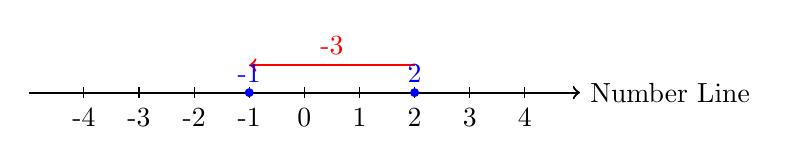
\begin{tikzpicture}[scale=0.7]
    \draw[thick,->] (-5,0) -- (5,0) node[right] {Number Line};
    \foreach \x in {-4,-3,...,4}
        \draw (\x,3pt) -- (\x,-3pt) node[below] {\x};
    \draw[red,thick,->] (2,0.5) -- (-1,0.5) node[midway,above] {-3};
    \filldraw[blue] (2,0) circle (2pt) node[above] {2};
    \filldraw[blue] (-1,0) circle (2pt) node[above] {-1};
\end{tikzpicture}
\end{center}

\subsection{Mental Math Strategies}
\begin{itemize}
    \item Rounding to the nearest 10 or 100
    \item Breaking numbers into easier parts
    \item Using the relationship between addition and subtraction
\end{itemize}

\section{Conclusion and Next Steps}
Mastering addition and subtraction lays the groundwork for more advanced mathematical concepts. As you become comfortable with these operations, you'll be ready to explore multiplication, division, and beyond.

\section{Challenge Problems}
\begin{enumerate}
    \item If you have 100 marbles and give away 15, then find 7 more, how many do you have?
    \item A store has 500 items. They sell 126 items on Monday and 89 items on Tuesday. How many items are left?
    \item You start with \$50. You spend \$13 on lunch, earn \$20 from babysitting, and then spend \$8 on a movie ticket. How much money do you have now?
\end{enumerate}

